This is about the smartcitizen NO2 results.

One SmartCitizen NO2 sensor was tested against the EPA reference.  It was 1 month old at the time of installation, and ran for 52 days (from 4/15 - 6/6 2016) with two ~40 minute service interruptions.  This test gave 74,961 samples of minute resolution data.


\subsection{Pre-processing}

Talk about process for taking raw aux/working electrodes and making the basic calibration data.


\begin{figure}[htb]
 	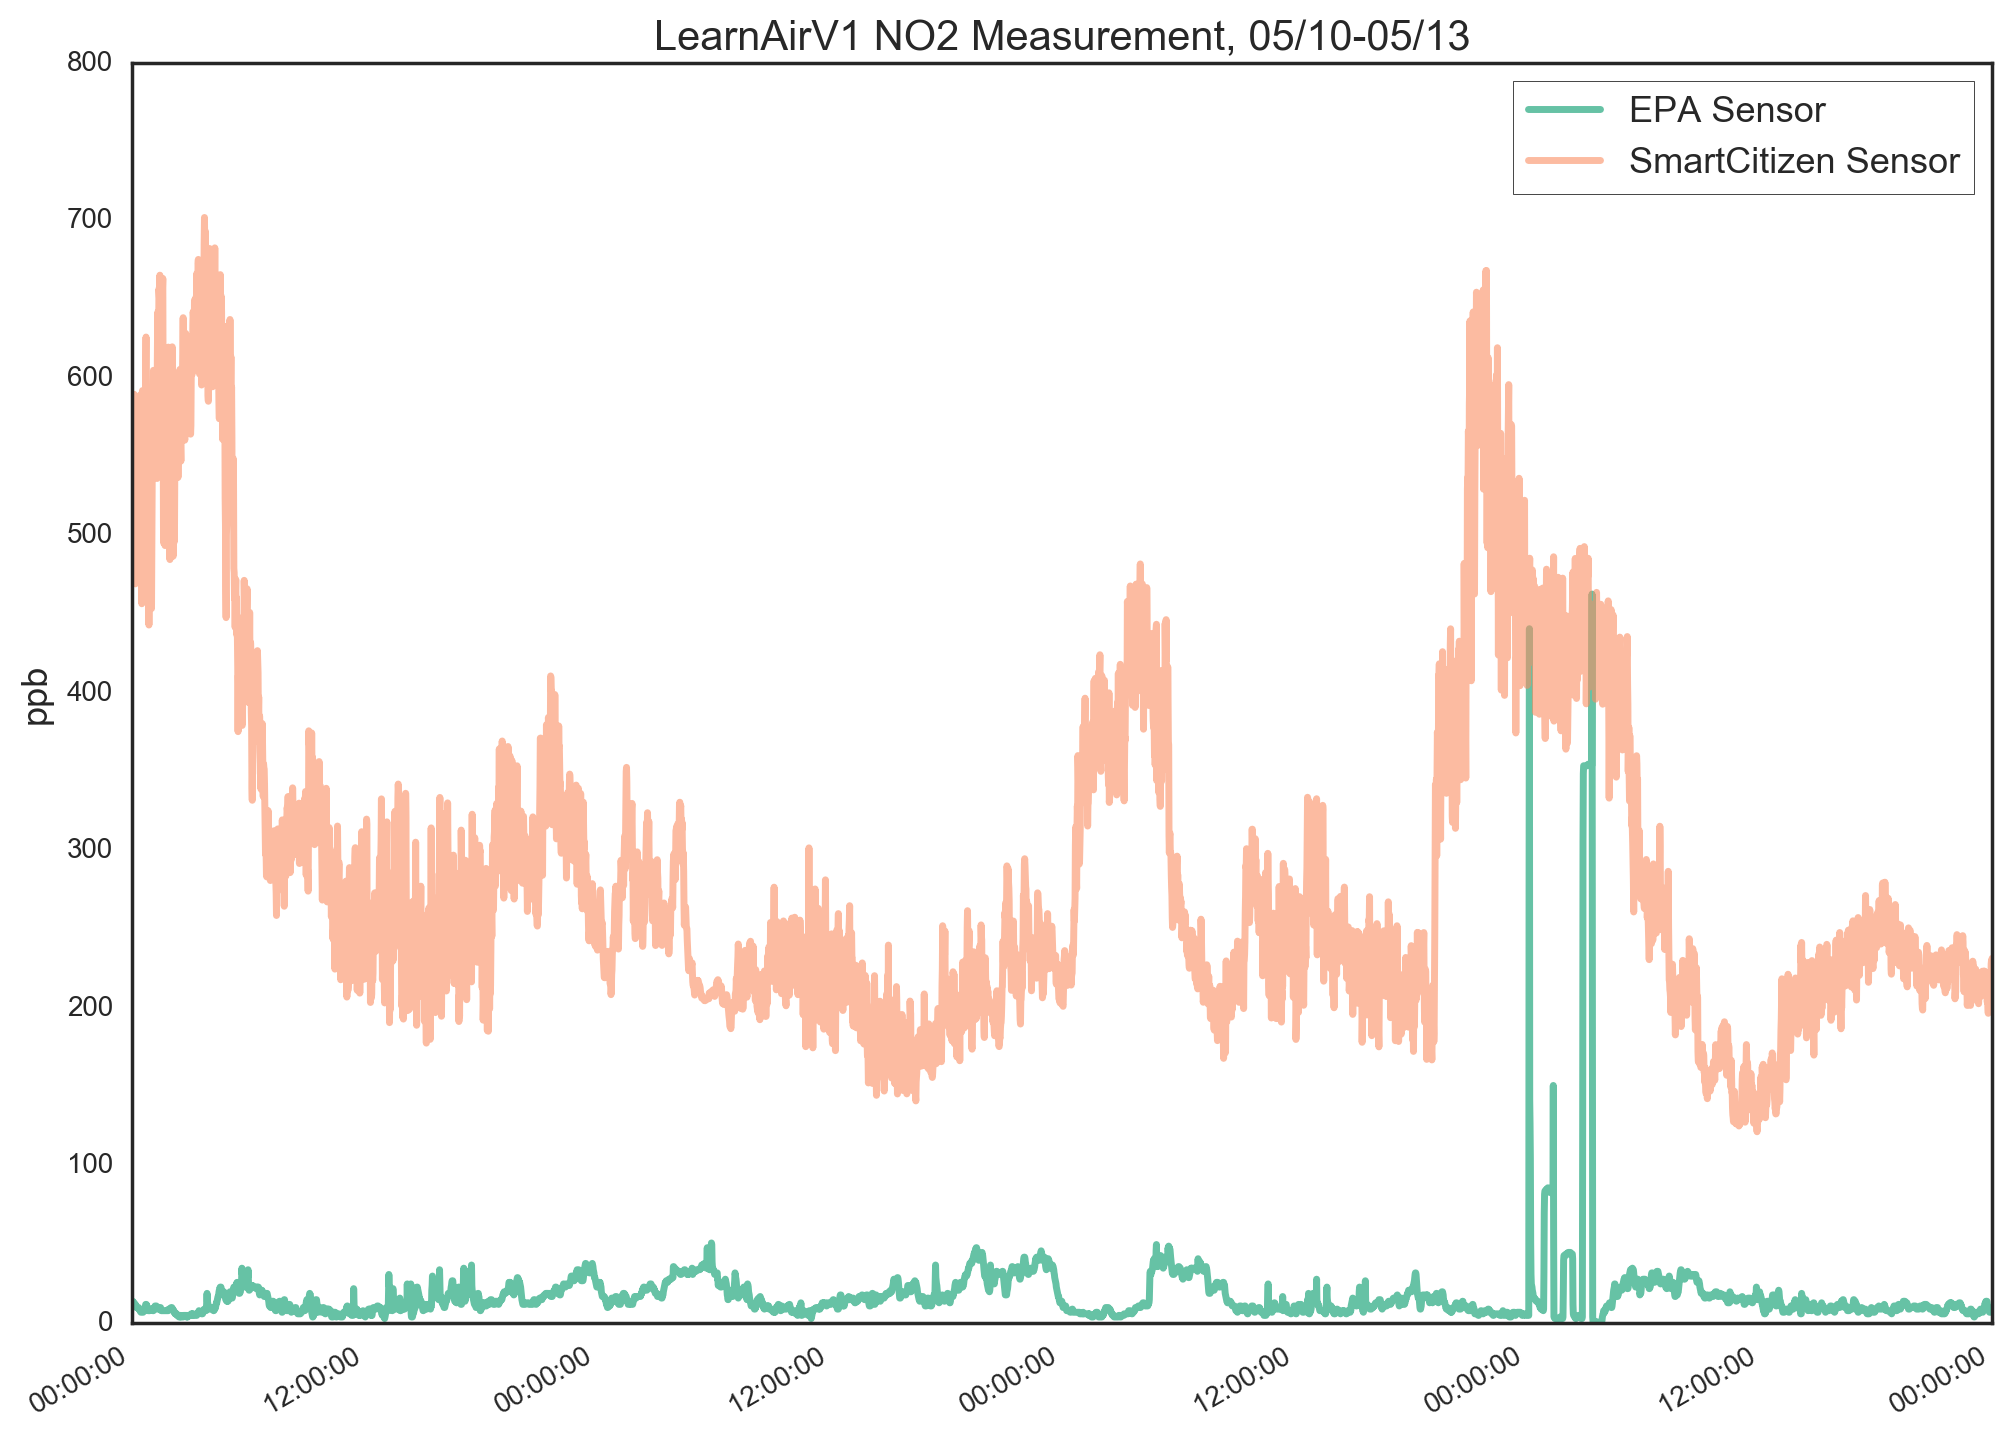
\includegraphics[width=\textwidth]{figs/no2_sck_zoomed}               
 	 \caption{SmartCitizen NO2 Raw Data}
  	\label{fig:sck_no2_raw_zoomed}
\end{figure}


\begin{figure}[htb]
 	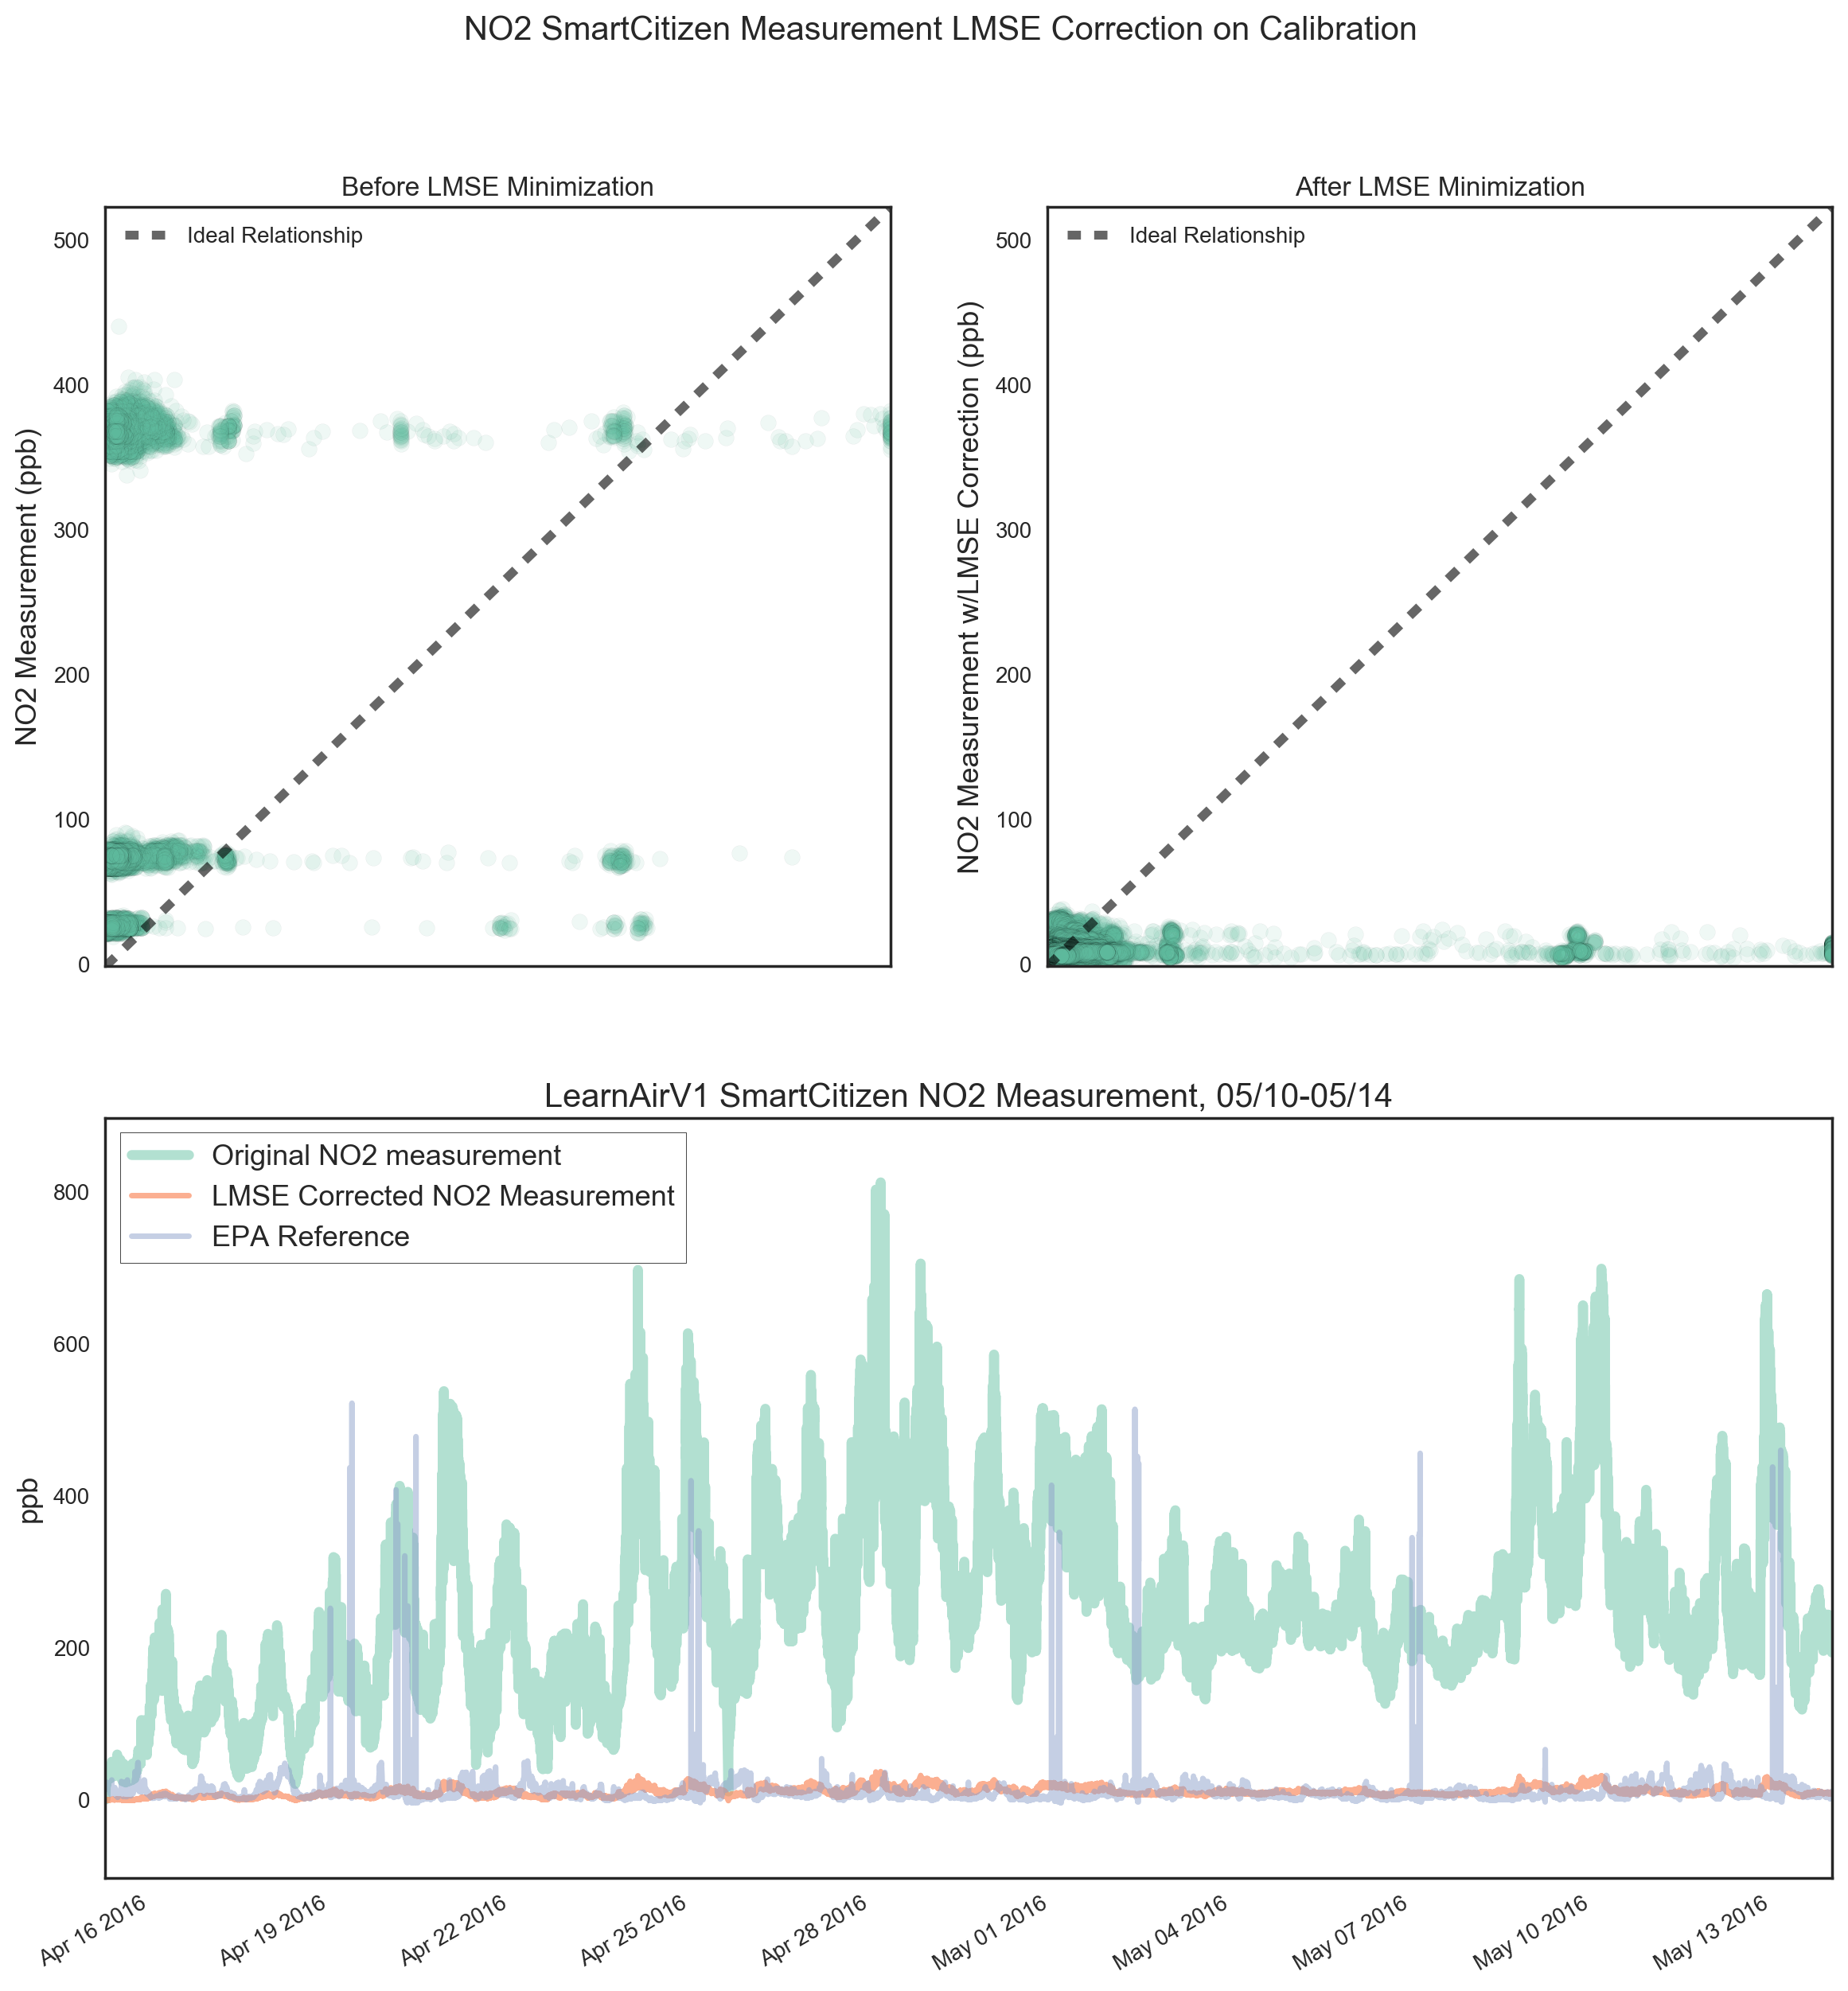
\includegraphics[width=\textwidth]{figs/sck_no2_lmse}               
 	 \caption{SmartCitizen NO2 after LMSE Calibration}
  	\label{fig:sck_no2_lmse}
\end{figure}








\subsection{Machine Learning}


\begin{figure}[htb]
 	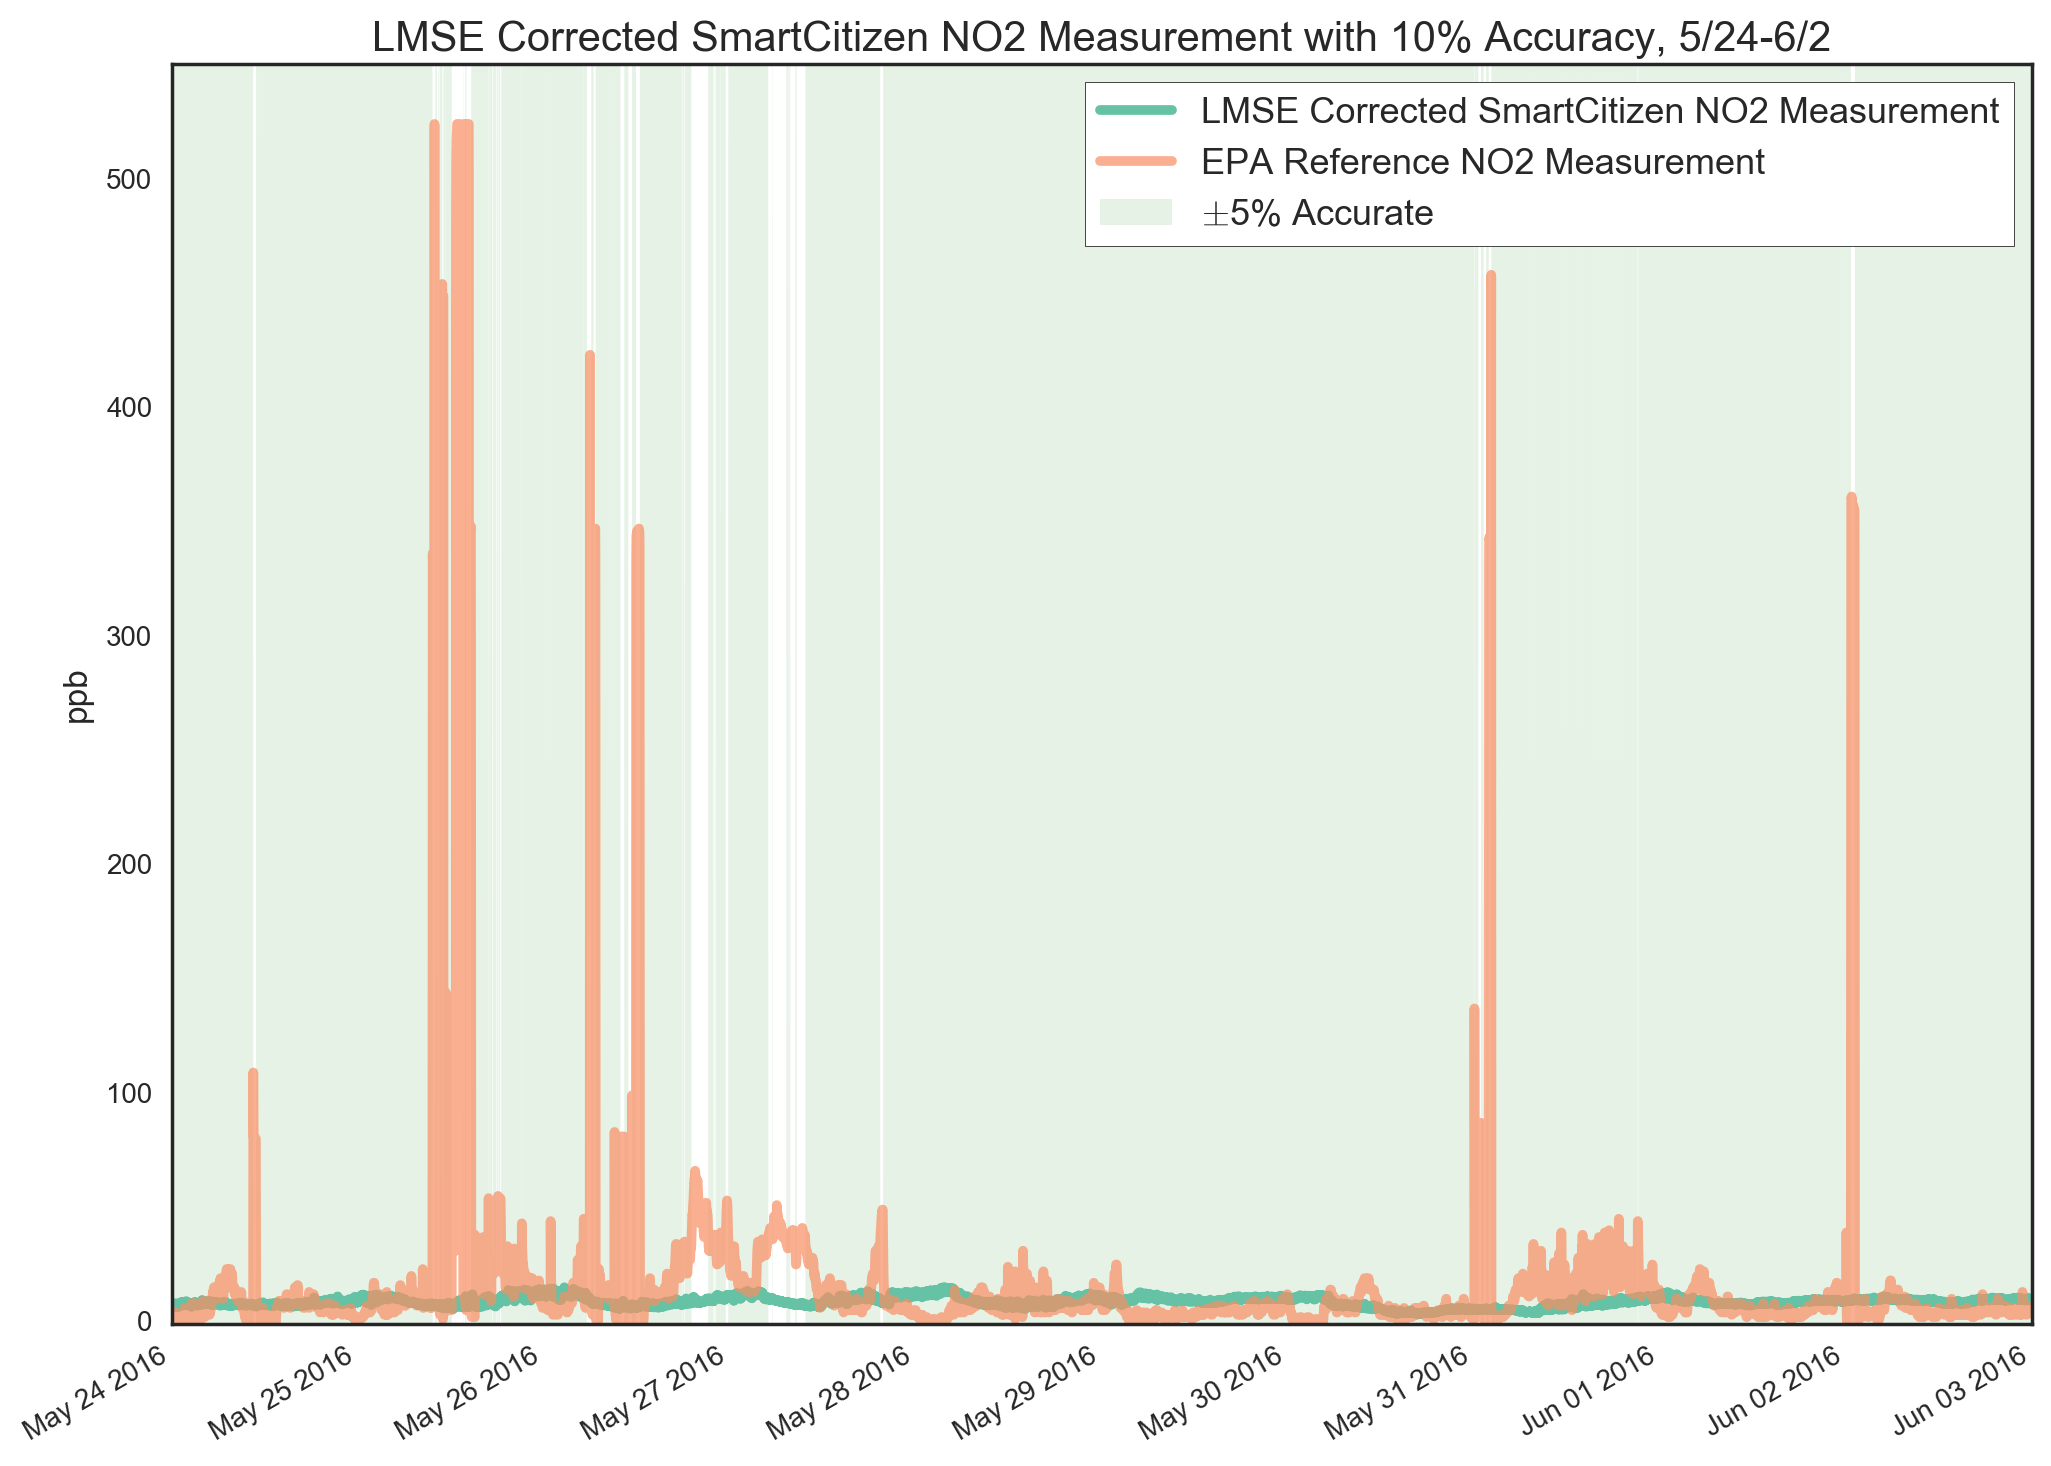
\includegraphics[width=\textwidth]{figs/sck_no2_with_10_accuracy_zoomed}               
 	 \caption{SmartCitizen NO2 with 10\% Accuracy Threshold}
  	\label{fig:sck_no2_with_10_accuracy_zoomed}
\end{figure}

\begin{figure}[htb]
 	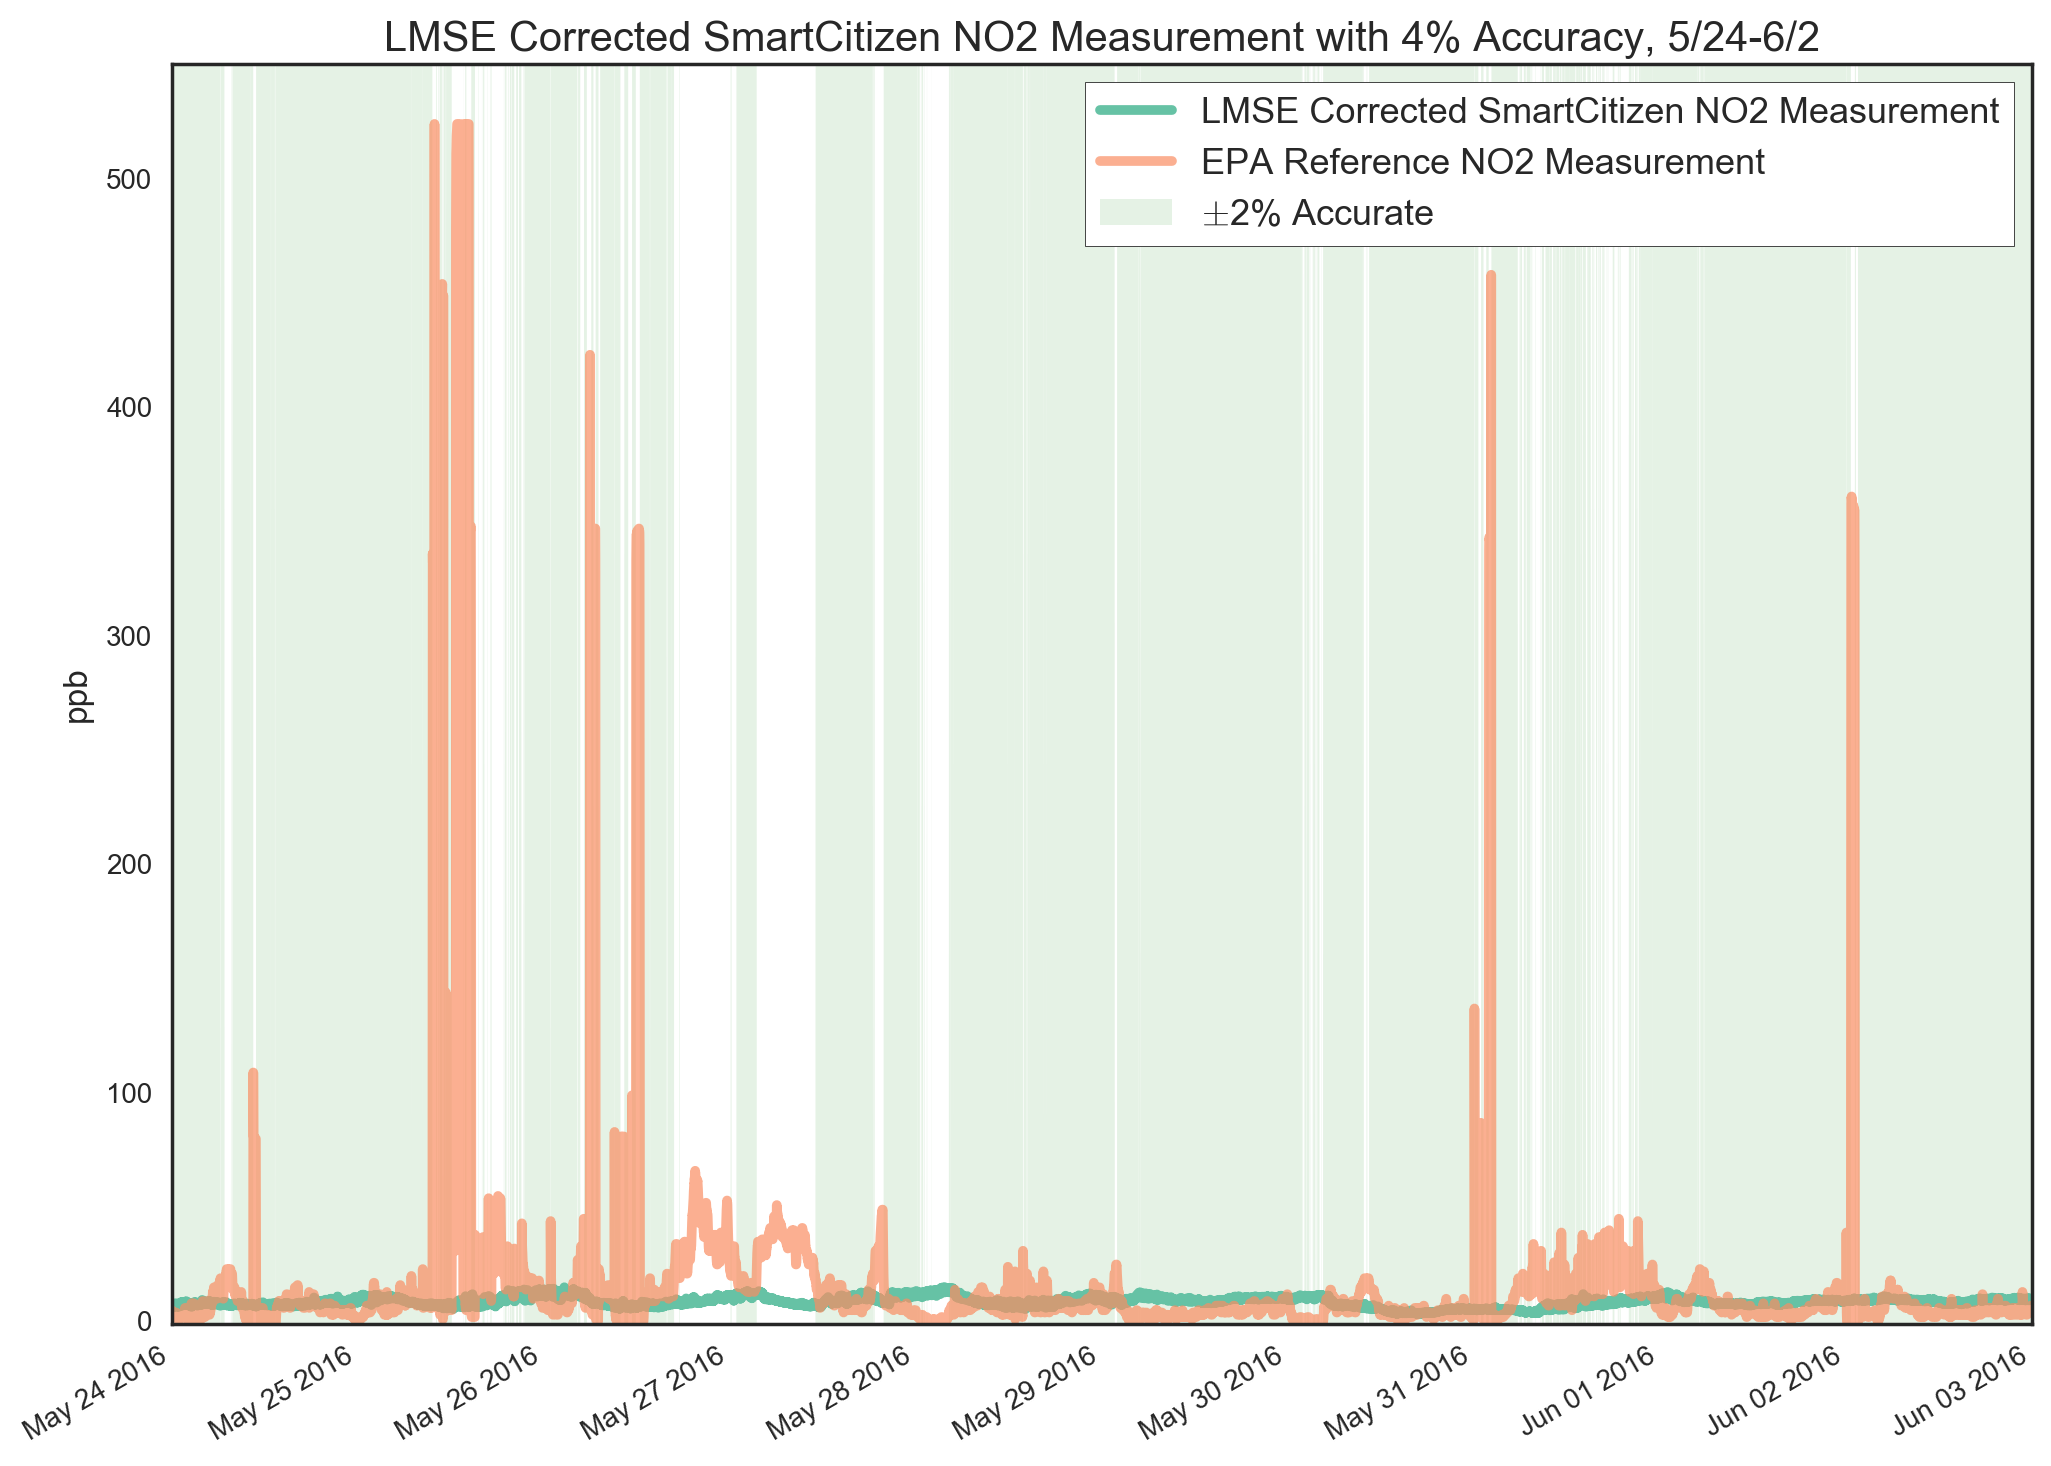
\includegraphics[width=\textwidth]{figs/sck_no2_with_4_accuracy_zoomed}               
 	 \caption{SmartCitizen NO2 with 4\% Accuracy Threshold}
  	\label{fig:sck_no2_with_4_accuracy_zoomed}
\end{figure}




%%%%

parameters = {'C':[0.001, 0.1, 10, 1000], 'penalty':('L1', 'L2') }

===== best ROC\_AUC score 0.907260610395

===== best params {'penalty': 'L1', 'C': 1000}



\begin{table}[H]
\centering
\begin{tabular}{|c|c|c|c|c|}
\toprule
\multicolumn{5}{|c|}{Error Rates for SmartCitizen NO2 with Logistic Regression} \\
&\multicolumn{2}{|c|}{all features} & \multicolumn{2}{|c|}{top 15 features} \\
&shuffled & chunked & shuffled & chunked \\
avg & 0.03 & 0.05 & 0.03 & 0.04 \\
min & 0.03 & 0.02 & 0.03 & 0.02 \\
max & 0.03 & 0.08 & 0.04 & 0.06 \\
\bottomrule
\end{tabular}
\label{tab:as1_co_error_rates}
\caption{Error Rates for Predicting SmartCitizen NO2 Accuracy with Logistic Regression}
\end{table}



\begin{margintable}[H]
\centering
\offinterlineskip
\hspace*{-5cm}\raisebox{-4cm}[0pt][0pt]{\rotatebox[origin=c]{90}{\parbox[c][0pt][c]{3cm}{\textbf{Actual Values}\\[20pt]}}}\par
\hspace{.3cm}\MyHBox[\marginparwidth]{Predicted Values}\par
\vspace{-.5cm}
\hspace*{1cm}\MyHBox{0}\MyHBox{1}\par
\MyTBox{0}{142.0}{427.0}
\vspace{-.35cm}\MyTBox{1}{52.6}{14370.2}\raisebox{-1cm}
}
\label{tab:sck_no2_confusion}
\caption{Average SmartCitizen NO2 Confusion Matrix w/Shuffled K-Fold}
\end{margintable}


\begin{figure}[htb]
 	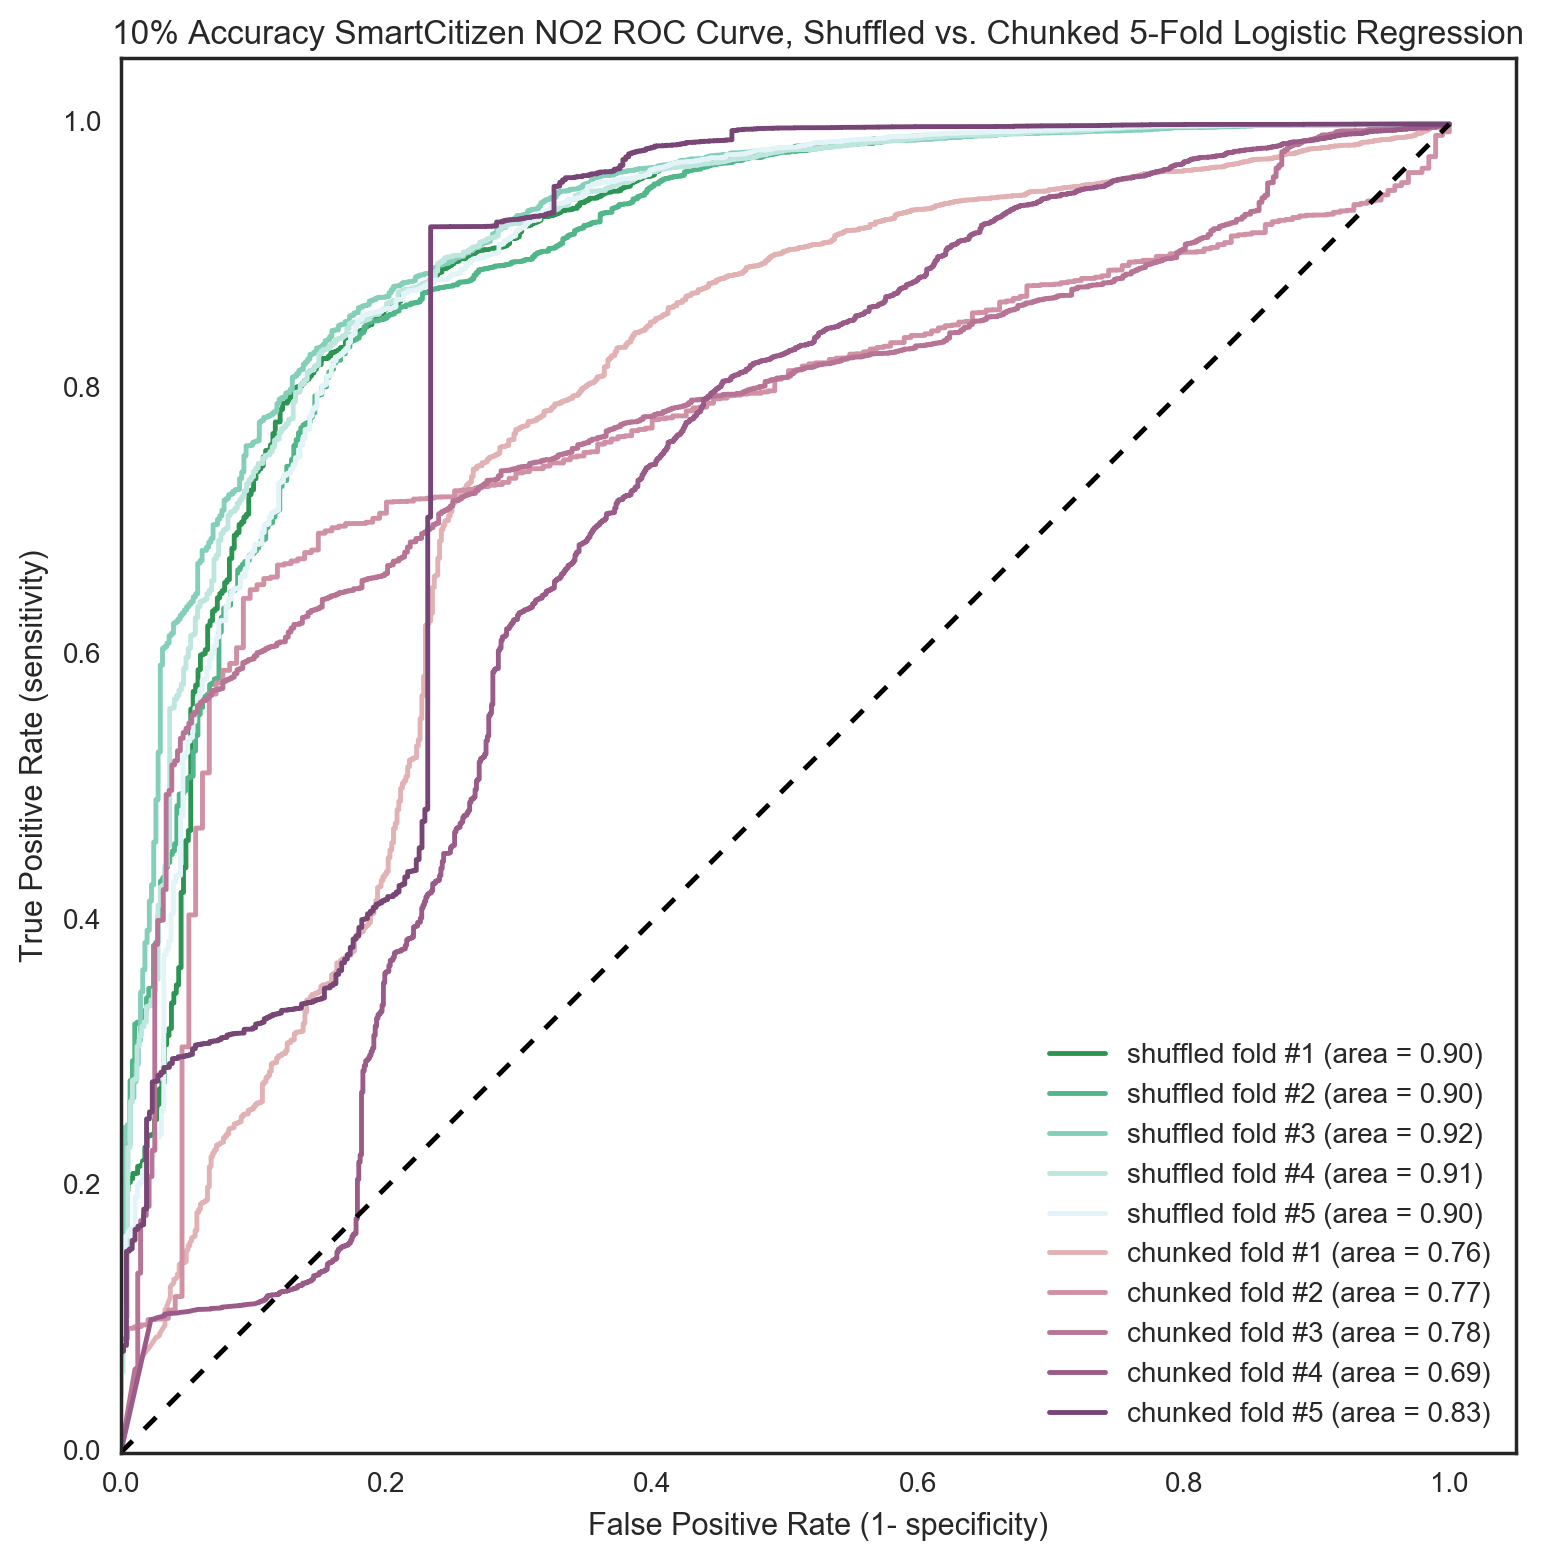
\includegraphics[width=\textwidth]{figs/sck_no2_10_roc}               
 	 \caption{SmartCitizen NO2 ROC Curve}
  	\label{fig:sck_no2_10_roc}
\end{figure}


here's text referencing the (Table \ref{tab:sck_no2_randomforest_features}).

\begin{table}[H]
\centering
\begin{tabular}{lllllllll}
\\
\\
\toprule
Feature & Importance \\
\midrule

bkcarbon & 0.0459890536212 \\
avg\_60\_bkcarbon & 0.0433384018273 \\
avg\_720\_bkcarbon & 0.024690468695 \\
avg\_1440\_bkcarbon & 0.0210702674105 \\
avg\_60\_forecastio\_windSpeed & 0.0207714428351 \\
min\_since\_plugged\_in & 0.0173782542533 \\
avg\_60\_forecastio\_windBearing & 0.0172875801677 \\
forecastio\_windSpeed & 0.0170176630128 \\
avg\_1440\_lmse\_calib\_as\_co & 0.0162266191466 \\
daily\_avg\_sck\_humidity & 0.0160827543221 \\
avg\_60\_forecastio\_pressure & 0.0157403595739 \\
avg\_720\_lmse\_scaled\_sharpDust & 0.0154263296837 \\
avg\_1440\_lmse\_scaled\_sharpDust & 0.0153038668128 \\
daily\_avg\_as\_temperature & 0.0151434934355 \\
daily\_avg\_forecastio\_temperature & 0.0148922895233 \\
\bottomrule
\end{tabular}
\label{tab:sck_no2_randomforest_features}
\caption{Top 15 Features from Random Forest for SmartCitizen NO2, used in Pruned Logistic Regression}
\end{table}



\begin{figure}[htb]
 	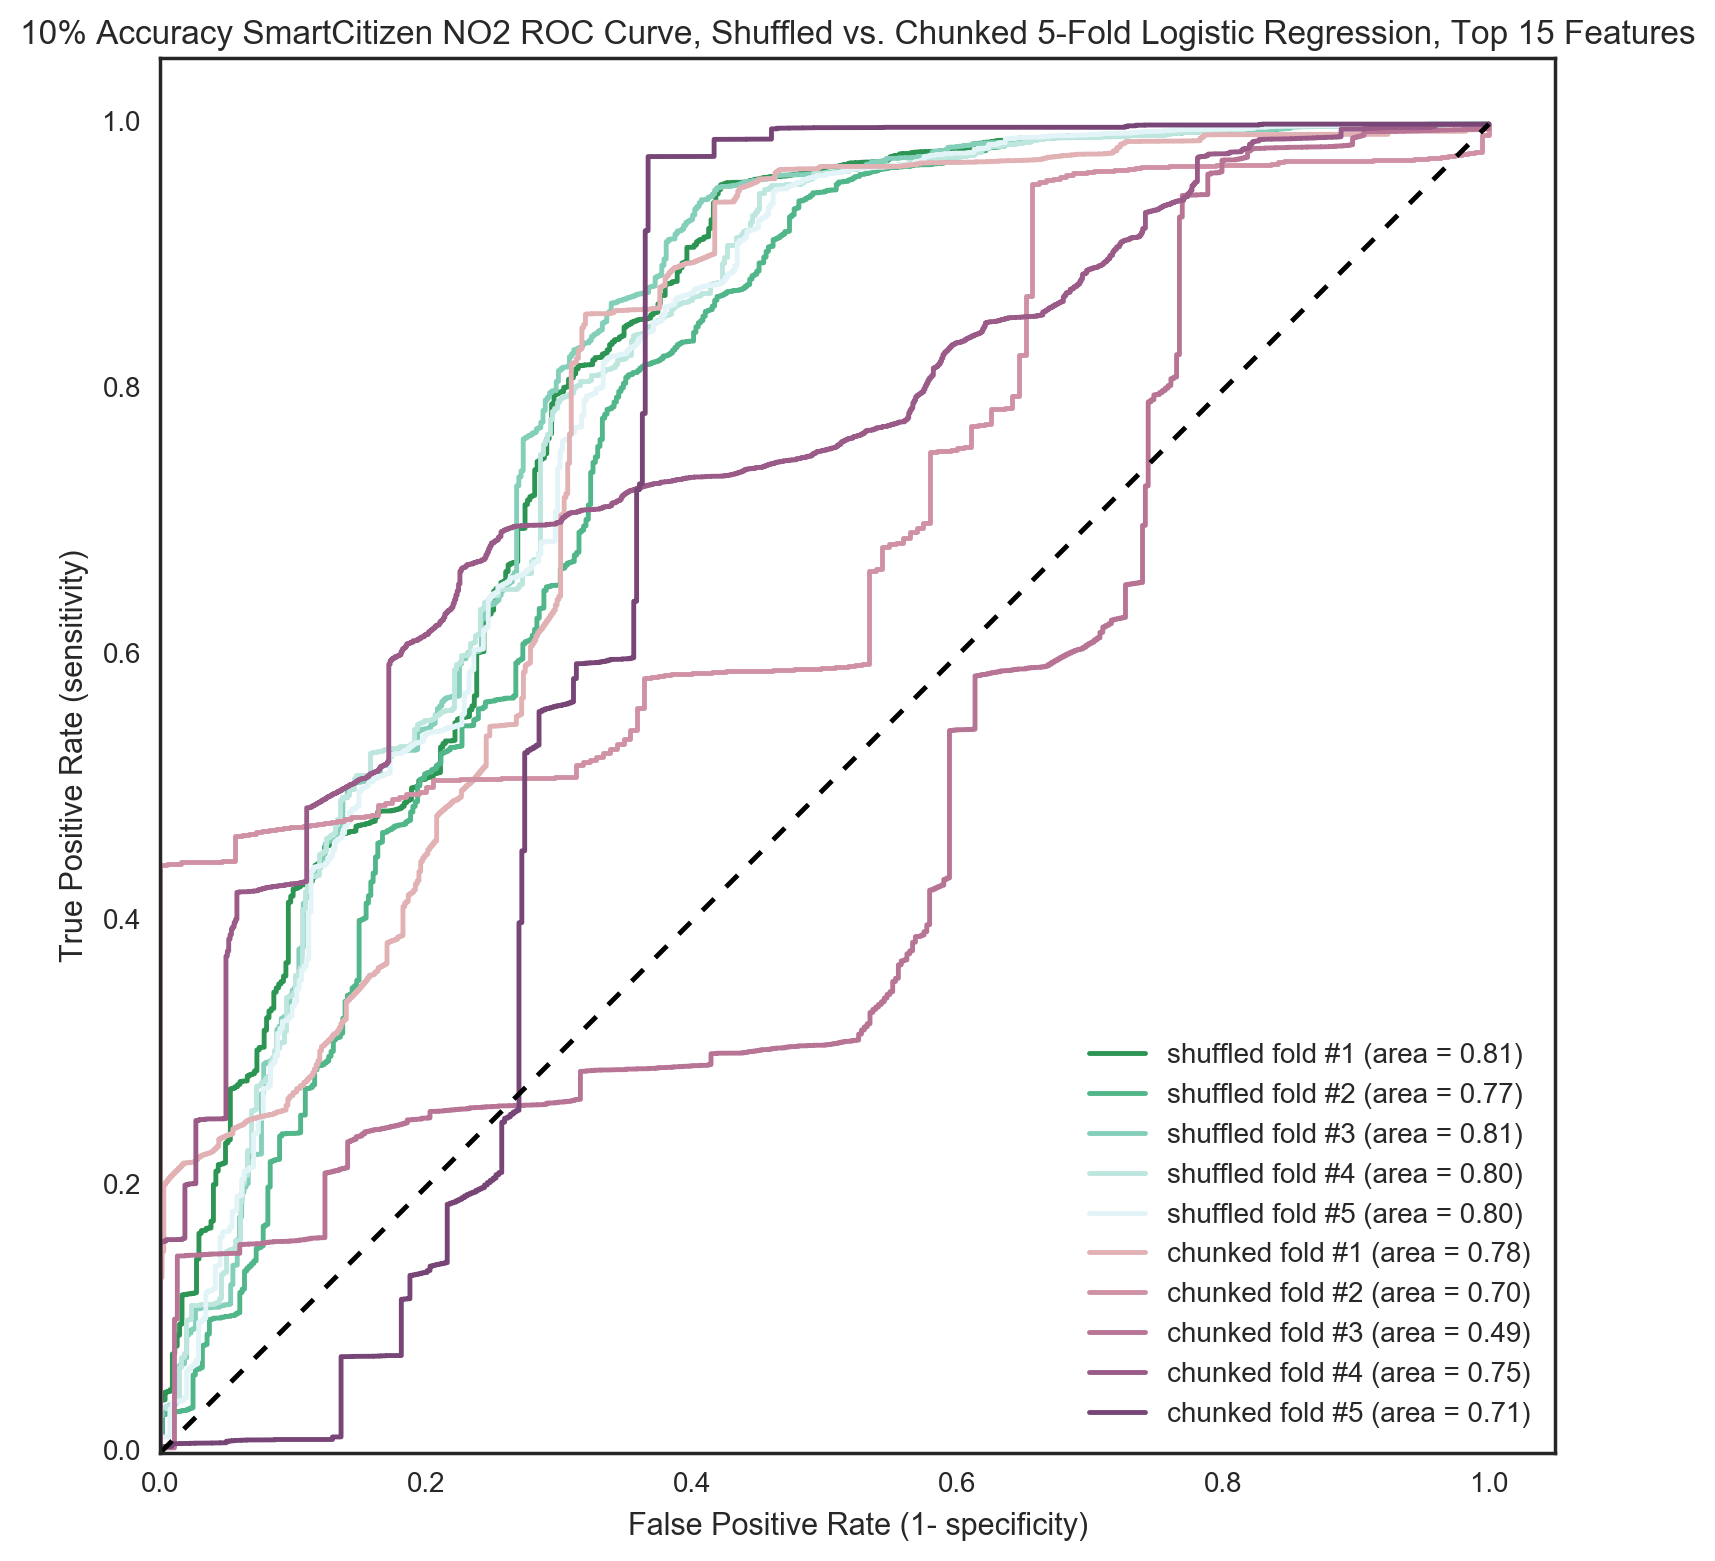
\includegraphics[width=\textwidth]{figs/sck_no2_10_roc_pruned_features}               
 	 \caption{SmartCitizen NO2 ROC Using Top 15 Features}
  	\label{fig:sck_no2_10_roc_pruned_features}
\end{figure}

\begin{figure}[htb]
 	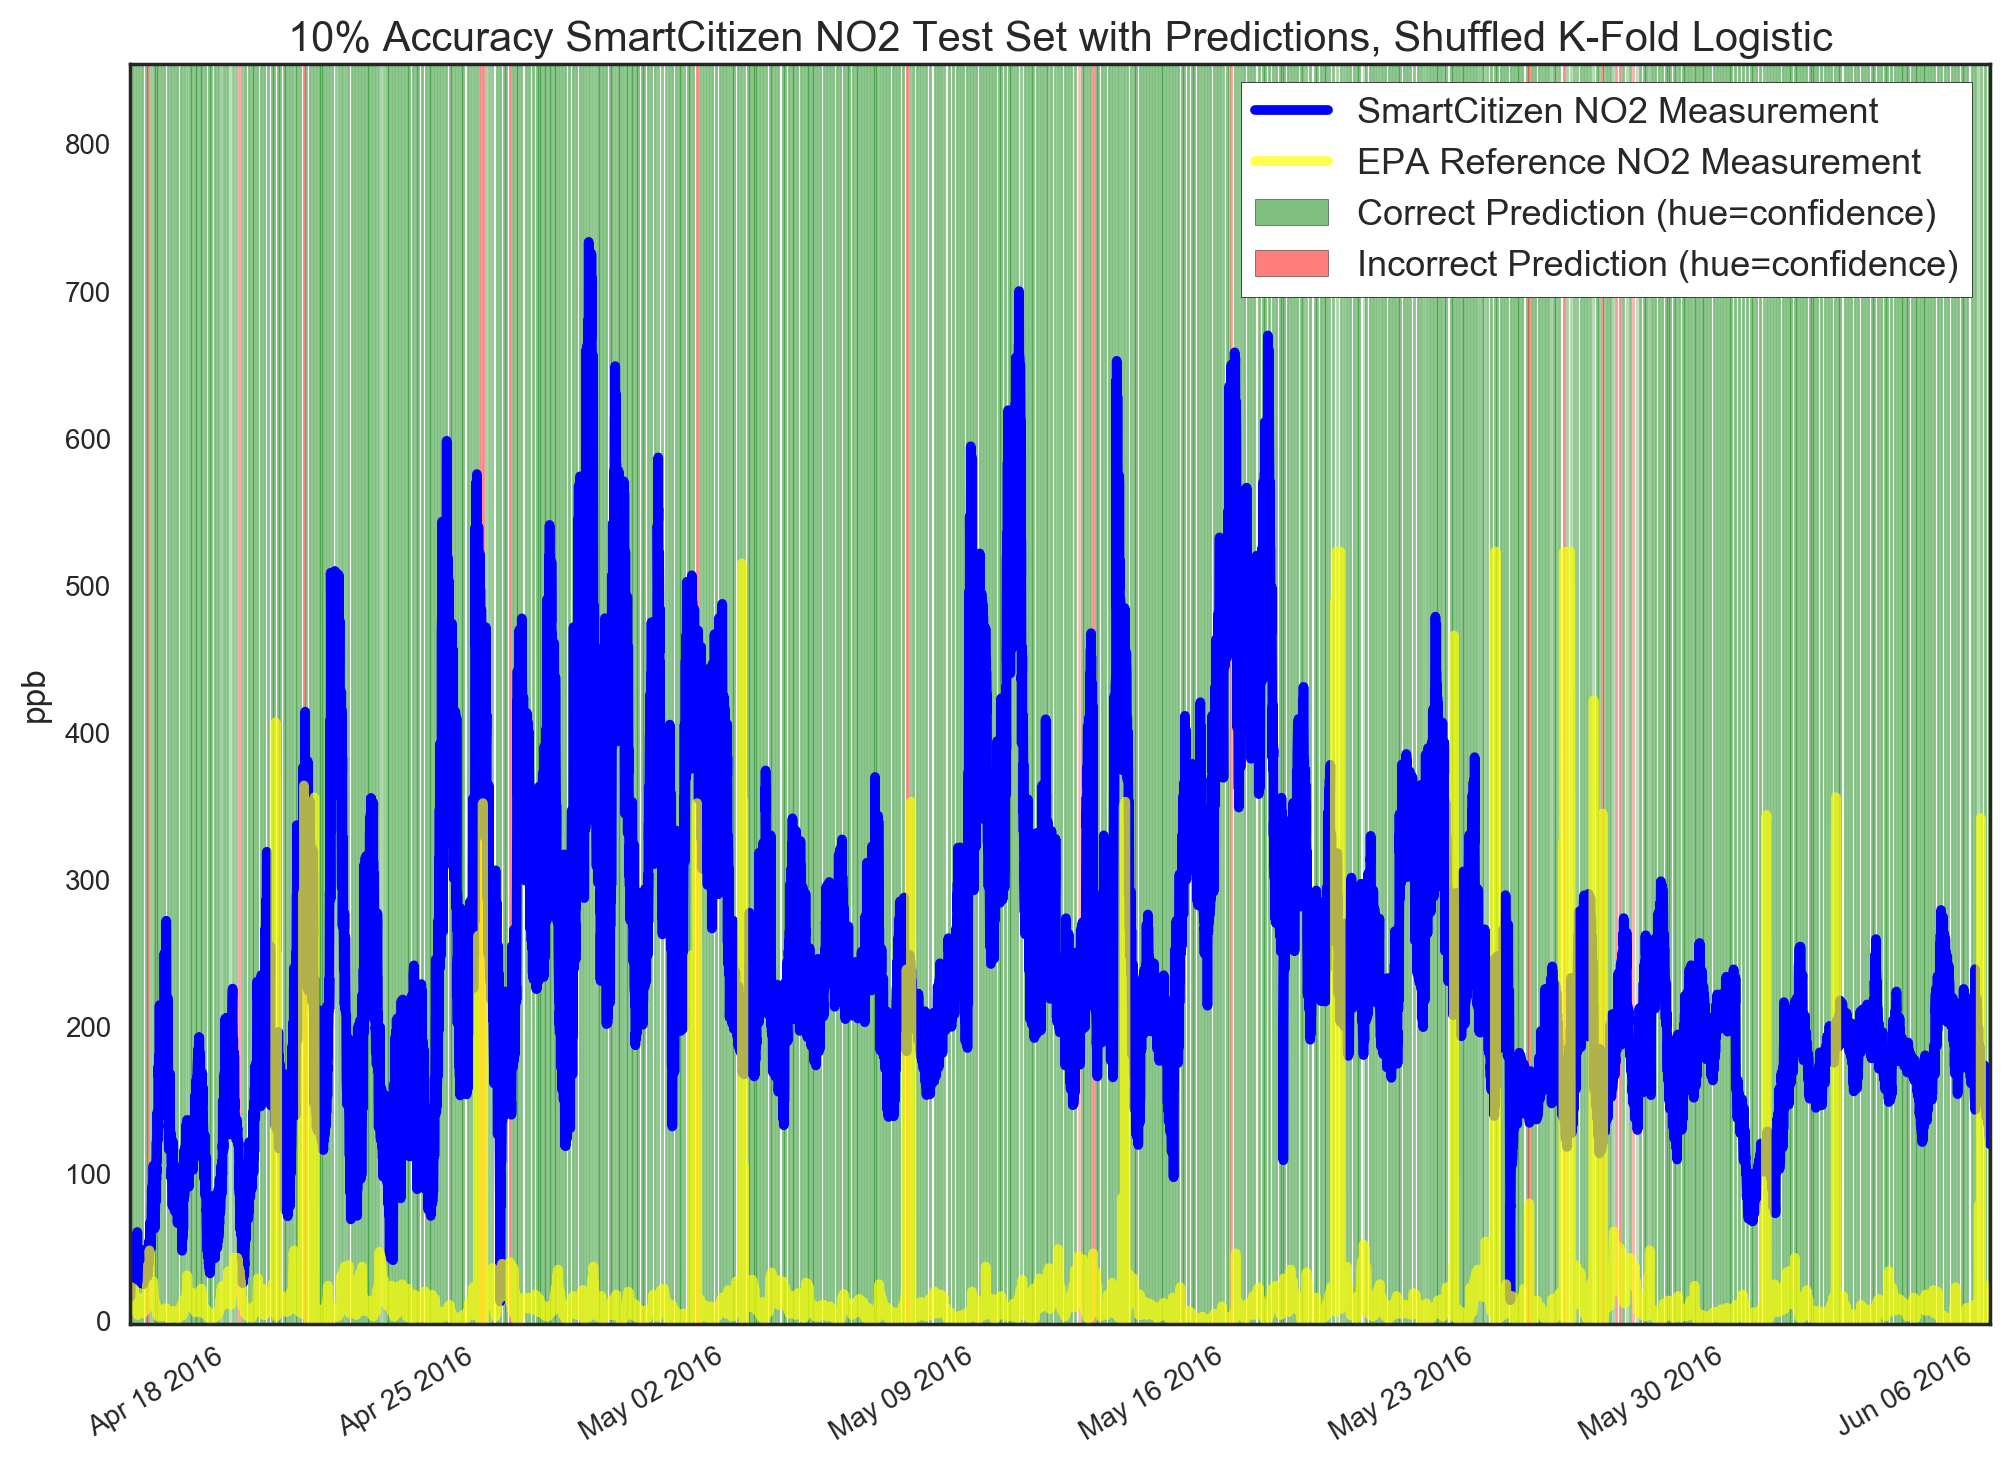
\includegraphics[width=\textwidth]{figs/sck_no2_10_logistic_predictions}               
 	 \caption{SmartCitizen NO2 Prediction Accuracy}
  	\label{fig:sck_no2_10_logistic_predictions}
\end{figure}



here's text referencing the (Table \ref{tab:sck_no2_top_features}).

\begin{table}[H]
\centering
\begin{tabular}{lllllllll}
\\
\\
\toprule
     & Corr. & Lasso & Lin Reg & RF   & RFE  & Ridge & Stability & Mean \\
\midrule
bkcarbon                                   & 1     & 0          & 0    & 1    & 0.63  & 0.51      & 0.85 & 0.57 \\
daily\_avg\_sck\_humidity                  & 0.11  & 0          & 0    & 0.32 & 0.67  & 1         & 0.76 & 0.41 \\
hour\_of\_day                              & 0.07  & 0.92       & 0    & 0.1  & 0.42  & 0.02      & 1    & 0.36 \\
avg\_60\_bkcarbon                          & 0.92  & 0          & 0    & 0.08 & 0.59  & 0.25      & 0.69 & 0.36 \\
derivative\_avg\_1440\_lmse\_calib\_as\_co & 0.06  & 0          & 0    & 0.05 & 0.62  & 0.38      & 1    & 0.3  \\
Solar Panel ( V)                           & 0.03  & 0          & 1    & 0    & 0.88  & 0         & 0    & 0.27 \\
lmse\_sck\_co                              & 0.01  & 1          & 0    & 0.02 & 0.85  & 0         & 0    & 0.27 \\
derivative\_avg\_1440\_bkcarbon            & 0.05  & 0          & 0    & 0.07 & 0.71  & 0.1       & 0.99 & 0.27 \\
humidity\_box\_differential                & 0.02  & 0          & 0.04 & 0.11 & 1     & 0.61      & 0    & 0.25 \\
forecastio\_partly-cloudy-night            & 0.03  & 0          & 0.16 & 0.02 & 0.95  & 0.11      & 0.42 & 0.24 \\
avg\_60\_forecastio\_humidity              & 0     & 0          & 0.04 & 0.06 & 1     & 0.61      & 0    & 0.24 \\
day                                        & 0.07  & 0          & 0    & 0    & 0.97  & 0.05      & 0.51 & 0.23 \\
night                                      & 0.07  & 0          & 0.01 & 0    & 0.98  & 0.05      & 0.43 & 0.22 \\
avg\_60\_forecastio\_precipProbability     & 0.04  & 0          & 0    & 0    & 0.6   & 0.49      & 0.44 & 0.22 \\
daily\_avg\_forecastio\_humidity           & 0.03  & 0          & 0    & 0.05 & 0.66  & 0.48      & 0.24 & 0.21 \\
forecastio\_rain                           & 0.03  & 0          & 0.16 & 0    & 0.9   & 0.25      & 0.04 & 0.2  \\
forecastio\_humidity                       & 0     & 0          & 0    & 0    & 0.64  & 0.72      & 0    & 0.19 \\
forecastio\_clear-night                    & 0.02  & 0          & 0.16 & 0    & 0.93  & 0.03      & 0.1  & 0.18 \\
forecastio\_fog                            & 0     & 0          & 0.16 & 0    & 0.9   & 0.21      & 0    & 0.18 \\
forecastio\_wind                           & 0.01  & 0          & 0.16 & 0    & 0.92  & 0.18      & 0    & 0.18 \\
avg\_720\_bkcarbon                         & 0.47  & 0          & 0    & 0.05 & 0.54  & 0.07      & 0.12 & 0.18 \\
avg\_30\_ws                                & 0.13  & 0          & 0    & 0.08 & 0.45  & 0.02      & 0.48 & 0.17 \\
avg\_15\_derivative\_sck\_temperature      & 0     & 0          & 0    & 0.04 & 0.63  & 0.5       & 0.01 & 0.17 \\
avg\_720\_lmse\_scaled\_sharpDust          & 0.01  & 0          & 0    & 0.16 & 0.58  & 0.41      & 0    & 0.17 \\
\bottomrule
\end{tabular}
\label{tab:as1_co_top_features}
\caption{Top Features for Predicting SmartCitizen NO2}
\end{table}


